%
% File: chap01.tex
% Author: Victor F. Brena-Medina
% Description: Introduction chapter where the biology goes.
%
\let\textcircled=\pgftextcircled
\chapter{Related Work}
\label{chap2}

\initial{D}ue to the large potential practical values in many domains and the big technical challenges, video analysis is a very hot research topic in both academic and industrial communities in recent years. Since the related works of interaction video analysis \cite{patron2010} \cite{Gemeren2015} \cite{narayan2014} \cite{choi2012} are relatively scarce compared with that in the closely related areas, like action video analysis \cite{Ji2013} \cite{Ng2015} \cite{Tran2015} \cite{alex2008} \cite{grepory2010} \cite{karpathy2014} \cite{simonyan2014}, we will both introduce the architectures used in interaction and action video analysis related works in Section \ref{2_1}. The general architecture of a video recognizer usually consists of a feature descriptor and a classifier. Video feature description research can be mainly divided into two directions: hand-crafted feature descriptors and learning based feature descriptors. We will introduce these two types separately in Section \ref{2_2} and \ref{2_3}. Another very important factor determines the performance of video analysis is the training datasets. Without rich and nicely annotated training dataset, it is hard to get a decent performance even for the best-built algorithm. So, we will introduce popular publicly available action and interaction video datasets in Section \ref{2_4}.

%=======
\section{Architectures of Interaction video analysis related works}
\label{2_1}
Choi et al. \cite{choi2012} introduce a hierarchical network to recognize the collective activity of a group of people. The hierarchical model is illustrated in Figure \ref{fig:hierA} (b). \(O_i\) and \(O_j\) are the features for each individual in the video, and \(O_c\) is crowd context feature which represents the overall information of the video. \(A\) is the atomic action for each individual, \(I\) is the interaction between two individuals and \(C\) is the collective activity of the group of people. For example, the collective activity \("gathering"\), illustrated in Figure \ref{fig:hierA} (a), is characterized as a collection of interactions (such as \("approaching"\)) between individuals. Each interaction is described as pairs of atomic activities (for example \("facing-right"\) and \("facing-left"\)). Each atomic activity is associated with a spatial-temporal trajectory. \cite{choi2012} use HOG to represent appearance features and use bag of video words (BoV \cite{bov}) to represent spatial-temporal features.
\begin{figure}
	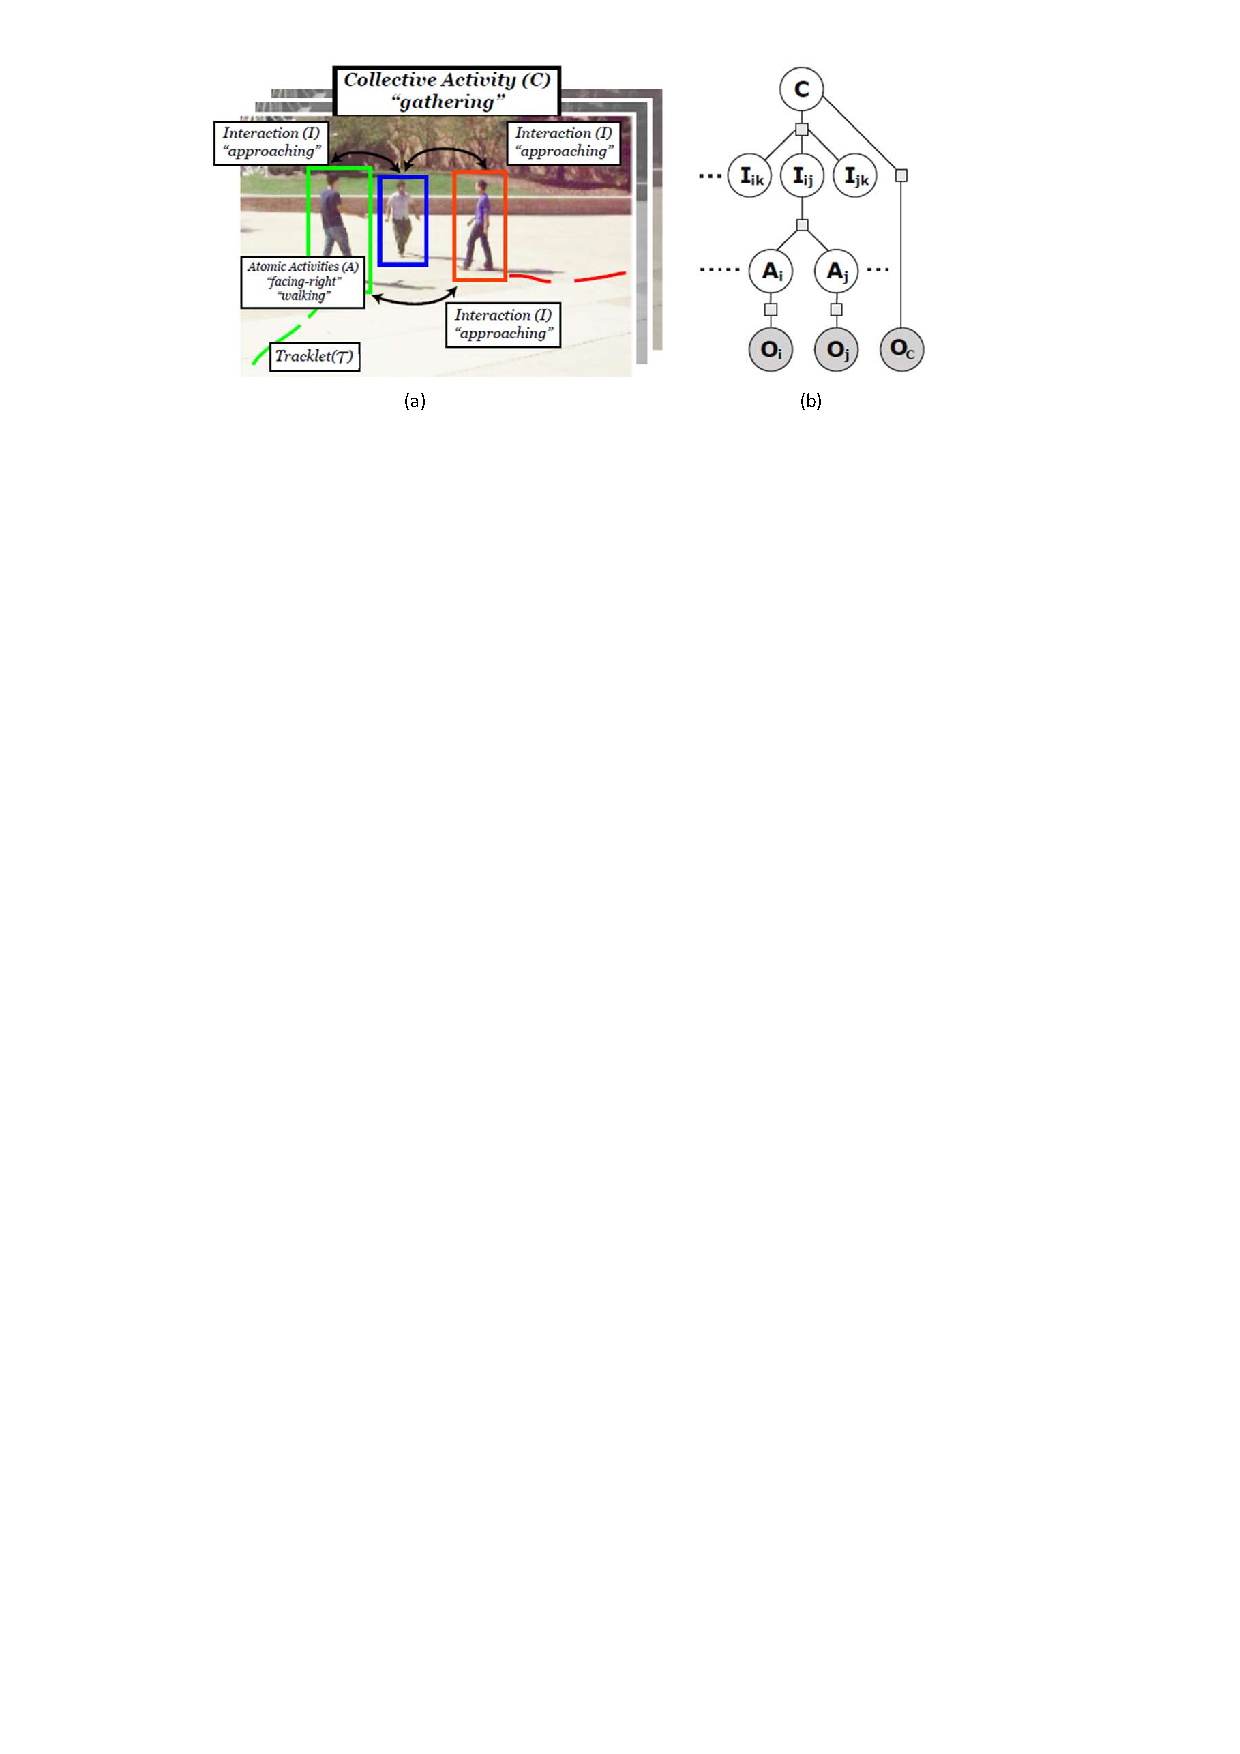
\includegraphics[trim=2cm 22.5cm 0cm 1cm]{figs/hier.pdf}
	\caption{The hierarchical activity recognition model and an example. Reprinted from \cite{choi2012}.}
	\label{fig:hierA}
\end{figure}
Compared with the work of Choi et al. which use hierarchical model to recognize group activities, Gemeren et al. \cite{Gemeren2015} extract interaction features from local body parts of interacting people and focus on those parts of videos that characterize the interaction. This is helpful to distinguish between interactions that differ only slightly. HOG (appearance) and HOF (movement) are combined as feature descriptors in this work.
\par
The work of Patron-Perez et al. \cite{patron2010} is similar with \cite{Gemeren2015}. Patron-Perez et al. detect and track the upper body for each person in the interaction video and crop the tracklet to generate a person-centred descriptor with HOG and HOF. Besides, the head orientation is also concerned in the feature descriptor because head orientation is also an important cue for interaction video analysis.
\par
There are also some methods which use bag of local features to describe the features of interaction, like the work of Yimeng et al. \cite{yimeng} and Yu et al. \cite{yu}. Yimeng et al. propose the concept of spatio-temporal phrase which is a combination of local features in a certain spatial and temporal structure including their order and relative positions, then the video is represented by a bag of spatio-temporal phrases. Yu et al. propose to use a set of attributes and the pair-wise co-occurrence relationship of two attributes to describe the videos. An attribute is a binary representation of a body part, like 'the torso is still'. A co-occurrence relationship of two attributes is a binary representation of the association between two attributes, for example, the co-occurrence relationships between attributes "torso bending" and "still leg" in the activity "bow". 

 

\section{Hand-crafted Feature Descriptor}
\label{2_2}

Scale-invariant feature transform (SIFT \cite{lowe1999} \cite{lowe2004})  and histogram of oriented gradients (HOG \cite{hog}) feature descriptors achieve great successes and are widely applied in the image content analysis. 
\par 
SIFT is a local feature describing algorithm which detects interest points in an image and computes the gradients for each interest point to construct features of an image. SIFT algorithm adopts difference of Gaussian (DoG) algorithm to detect the interest points by constructing an image pyramid with several scales and blurring images with several different Gaussian filters for each scale. The interest points are those points with maximum values compared with their neighbor pixels in the image pyramid. Thus, those points with edges and corners which represent the main feature of an object are most likely to be found as interest points. Because interest points are detected in different scales, SIFT feature descriptor is scale invariant.  Gradient computing is applied for the interest point centered blocks for each interest point. The computed histogram of gradient features are rotated to the main orientation for each interest point, thus it is rotation invariant. At last, the features are normalized to further eliminate the effect of different lighting.
\par 
For HOG algorithm, the image is divided into several small cells, histogram of gradient ( orientation and magnitude) are computed for each cell. This is because the appearance and shape of an object can be nicely described by the gradient. HOG feature descriptor is somewhat transform invariant because the features are computed in local cells. And because the features are normalized over sliding overlap blocks which contain several cells in a block. So, it is lighting invariant.
\par
Though SIFT and HOG can efficiently describe appearance and shape features for images, but they can not be directly used for video analysis task, because the video analysis requires not only appearance and shape description but also motion description. Thus, they are also extended to 3D-SIFT\cite{grepory2010} \cite{paul2007} and 3D-HOG\cite{alex2008} to describe the video features. Among all current hand-crafted feature descriptors, improved Dense Trajectories(iDT)\cite{wang2012}\cite{wang2013} have been shown to perform best on a variety of datasets. 

\subsection{3D-SIFT Feature Descriptor}
\label{2_2_1}
Compared with 2D-SIFT\cite{lowe1999}\cite{lowe2004} which only considers x and y dimensions, 3D-SIFT\cite{grepory2010}\cite{paul2007} takes another time(t) dimension into consideration, because the motion information contained in time dimension is an essential cue for video analysis. There are two steps to construct the SIFT feature descriptor. The first step is key points localization and the second step is calculating the sub-histograms for each key point. The method of key points localization is as same as 2D-SIFT. The main differences between 2D-SIFT and 3D-SIFT is calculating the sub-histogram for each key point.
\par 
The 2D gradient magnitude and orientation for each pixel are calculated in \(x\) and \(y\) dimensions while 3D-SIFT calculates gradients in three dimensions \(x\), \(y\) and \(t\). Thus, the motion information along the time dimension is also well presented by the sub-histogram of 3D gradients.  
\begin{figure}
	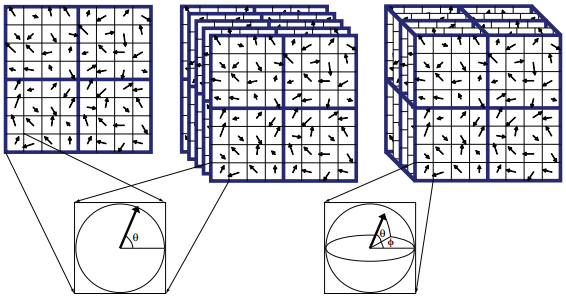
\includegraphics[width=\linewidth]{figs/3D_SIFT.png}
	\caption{The SIFT descriptor. The left image shows the 2D SIFT descriptor. The center image shows how multiple 2D SIFT descriptor could be used on a video without modification to the original method. The right image shows the 3D SIFT descriptor with its 3D sub-volumes, each sub-volume is accumulated into its own sub-histogram. These histograms are what makes up the final descriptor. Reprinted from \cite{grepory2010}.}
	\label{fig:3DSIFT}
\end{figure}
\par 
The 3D-SIFT feature descriptor is illustrated in Figure \ref{fig:3DSIFT}. After getting the sub-histogram, the orientation of each key point could be fixed. In 3D-SIFT, the dominant orientation of key point could be represented by\(\) \(\theta\) and \(\phi\). To keep the orientation invariant, all neighbourhood of each key point are rotated to the dominant orientation. 3D-SIFT also inherits the method of key points detection and histogram normalization from 2D-SIFT, thus, it is also scale and lighting invariant. 


\subsection{3D-HOG Feature descriptor}
\label{2_2_2}
2D-HOG is widely used for the purpose of object detection in static images. 2D-HOG calculates the gradient orientation for each pixel and statics them as histogram of orientated gradient over cells. Klaser et al. extended it to 3D-HOG\cite{alex2008}. In Klaser's work, the main differences between 2D and 3D HOG is the calculation of gradient. In 2D-HOG, only two dimensions \(x\) and \(y\) are considered, the cell is a square. While in 3D-HOG, additional time dimension \(t\) is taken into consideration, so, the cell is a cube. The blocks which used to contrast-normalization also became from 2D square to 3D cube. The overview of the descriptor computation is illustrated in Figure \ref{fig:3DHOG}.
\begin{figure}
	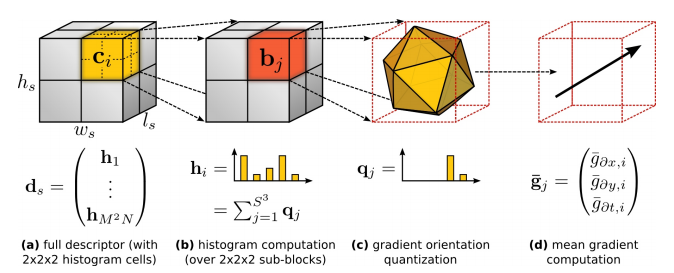
\includegraphics[width=\linewidth]{figs/3D_HOG.png}
	\caption{ Overview of 3D-HOG descriptor computation; (a) the support region around a point
		of interest is divided into a grid of gradient orientation histograms; (b) each histogram is
		computed over a grid of mean gradients; (c) each gradient orientation is quantized using
		regular polyhedrons; (d) each mean gradient is computed using integral videos. Reprinted from \cite{alex2008}.}
	\label{fig:3DHOG}
\end{figure}
\par 

For the similar reason as that in 3D-SIFT, 3D-HOG calculates gradients in both spatial and temporal dimensions, so, the motion information contained in the time dimension can be nicely represented by 3D-gradients. 

\subsection{Improved Dense Trajectories feature descriptor}
\label{2_2_3}

Improved Dense Trajectory (iDT) is a very successful algorithm for video action recognition among all hand-crafted feature descriptors which was proposed by Wang et al. \cite{wang2012} \cite{wang2013}.  \cite{wang2012} introduces the Dense Trajectory (DT) algorithm and \cite{wang2013} improves DT algorithm by eliminating background optical flow trajectory caused by camera motion.
\par
The overview of DT feature descriptor is illustrated in Figure \ref{fig:DT}, including dense sampling, key points tracking and features description. The video is firstly extended to several different spatial scales to keep this feature descriptor scale invariant.
\par 
Feature points are densely sampled on a grid spaced by \(W\) pixels. Sampling is carried out on each spatial scale separately. Since it is hard to track feature points in homogeneous areas, Wang et el. remove those points which have very small eigenvalues of the auto-correlation matrix. 
\par 
Feature points are tracked on each spatial scale separately. Given a point \(P_t = (x_t,y_t)\) in frame \(I_t\), its tracked position in frame \(I_{t+1}\) is calculated by the position in frame \(I_t\) and the the components of optical flow computed  w.r.t. \(I_t\) and \(I_{t+1}\). Due to the fact that it is unstable to track a feature point in long time, all the feature points are re-sampled every \(L\) frames. Then for every feature point, the trajectory feature vector is \((P_t,P_{t+1},P_{t+2}....,P_{t+L-1})\). The trajectory feature vector contains motion information of feature points thus it can represent motion information for videos. 
\par 
Since only trajectory features are not enough to describe all the video features, Wang et al. introduce another three feature descriptors: Histograms of Orientated Gradient (HOG \cite{hog}), Histograms of Optical Flow (HOF \cite{hof} and Motion Boundary Histograms (MBH \cite{hof}). The HOG feature descriptor is similar with 3D-HOG but it is calculated along trajectory. HOF features represent the optical flow (movements) of objects in videos and MBH features are based on derivatives of optical flow which is a simple and effective way to suppress camera motion. 3D-HOG can well represent the both appearance/shape and motion information for objects in videos. The combination of HOF and MBH can further improve the video analysis performance as they represent zero-order (HOF) and first-order (MBH) motion information. All of these three feature descriptors are calculated in a \(N*N*L\) spatial-temporal volume around the feature point along the trajectory, see the right image in Figure \ref{fig:DT}. The spatial-temporal volume is sliced into smaller \(n\sigma * n\sigma * n\tau \) spatial-temporal cells. \(N= 32, n\sigma = 2, n\tau = 3 \) in the work of Wang et al. The histogram of HOG, HOF and MBH are calculated over all pixels in each cell.

\begin{figure}
	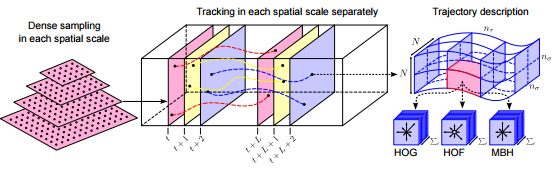
\includegraphics[width=\linewidth]{figs/DT.png}
	\caption{Illustration of DT algorithm to extract and characterize dense trajectories. Left: Feature points
		are densely sampled on a grid for each spatial scale. Middle: Tracking is carried out in the corresponding
		spatial scale for L frames by median filtering in a dense optical flow field. Right: The trajectory shape
		is represented by relative point coordinates, and the descriptors (HOG, HOF, MBH) are computed along
		the trajectory in a \(N * N\) pixels neighbourhood, which is divided into \(n\sigma * n\sigma * n\tau \) cells. Reprinted from \cite{wang2012}.}
	\label{fig:DT}
\end{figure}
 
\par 
The work of iDT \cite{wang2013} improves DT algorithm mainly by eliminating the camera motion. In DT algorithm, due to the camera motion, there are many trajectories in the background, and the trajectories of interest can also be affected by the camera motion. But those trajectories of background are unuseful for action recognition and usually confuse the results. By assuming the difference between 2 consecutive frames is small, the iDT algorithm assumes that the frame \(I_{t+1}\) can be calculated from frame \(I_t\) and a transform matrix \(H\), that \(I_{t+1} = I_t * H \).  Then we can calculate \(Iwarp_{t+1} = H^{-1} * I_{t+1}\), where \(Iwarp_{t+1}\) is the frame \(I_{t+1}\) after eliminating camera motion. Since the transformation matrix \(H\) is calculated over the whole image \(I_t\) and \(I_{t+1}\) which include both background and interest human. So, the large movement of human body in consecutive frames will largely affect the accuracy of matrix \(H \). Wang et al. use human detection technique to detect the human body in all images and mask these areas to get more accurate transform matrix \(H\) and use this matrix to eliminate useless trajectory of background and human body caused by camera motion.

\section{Deep Learning Based Feature Descriptor}
\label{2_3}

Though hand-crafted feature descriptors achieve very nice performance in image and video content analysis, they are all based on pre-defined rules to extract features. Thus, they usually ignore those potential cues for video analysis which not be realized by the feature designer. A deep learning based feature descriptor has complex parameters and flex structure. A well trained deep learning feature descriptor can represent similar features represented by hand-crafted feature descriptor. For example, Convolutional Neural Network (CNN or ConvNet \cite{cnn}) can learn edges in lower layer which is similar with HOG. Further, well trained deep learning feature descriptor has potential abilities to represent some features which are hard for hand-crafted features descriptors. That is learning feature descriptor is more general than hand-crafted feature descriptor.  Due to the significant development of data science, deep learning based feature descriptor, especially CNN,  shows powerful ability of feature representation and has achieved state of art performance in image classification/recognition \cite{kaiming}.
\par 
Convolutional Neural Network is one type of deep artificial neural network in which the connectivity pattern between its neurons is inspired by the organization of animal visual cortex. The architecture of one of the very first ConvNet, LeNet5 by Yann LeCun et al. \cite{cnn}, is illustrated in Figure \ref{fig:cnn}. A typical ConvNet includes three main parts: convolutional layers, pooling/subsampling layers and fully connected layers. Convolutional layers extract features from input image by applying convolution. The convolution can be understood as a feature filter applying over the input image. We can perform operations such as edge detection just by setting different filter parameters. So, one filter (convolutional kernel) can extract one type of features. The more filters, the more features can be represented by the ConvNet. An intuitive example of convolution is illustrated in Figure \ref{fig:conv}. The pooling/subsampling layer reduces the dimensionality of each feature map but retain the most import information. There are different types of pooling: Max which takes the largest element in a \(n \times n\) window; and Average which takes the average value of all elements in the window. Pooling operation can simplify the features thus has following advantages: 1). Making the network smaller and more manageable; 2). Reducing the number of parameters and computation, therefore controlling over-fitting; 3). Making the network invariant to small transformations, distortions, etc. Fully connected layer is a traditional multi layer perceptron in which every neuron in the previous layer is connected to every neuron on the next layer. The output of convolutional and pooling layers represents high-level features of input images while the fully connected layers use these features to classify these input images into various classes.  

\begin{figure}
	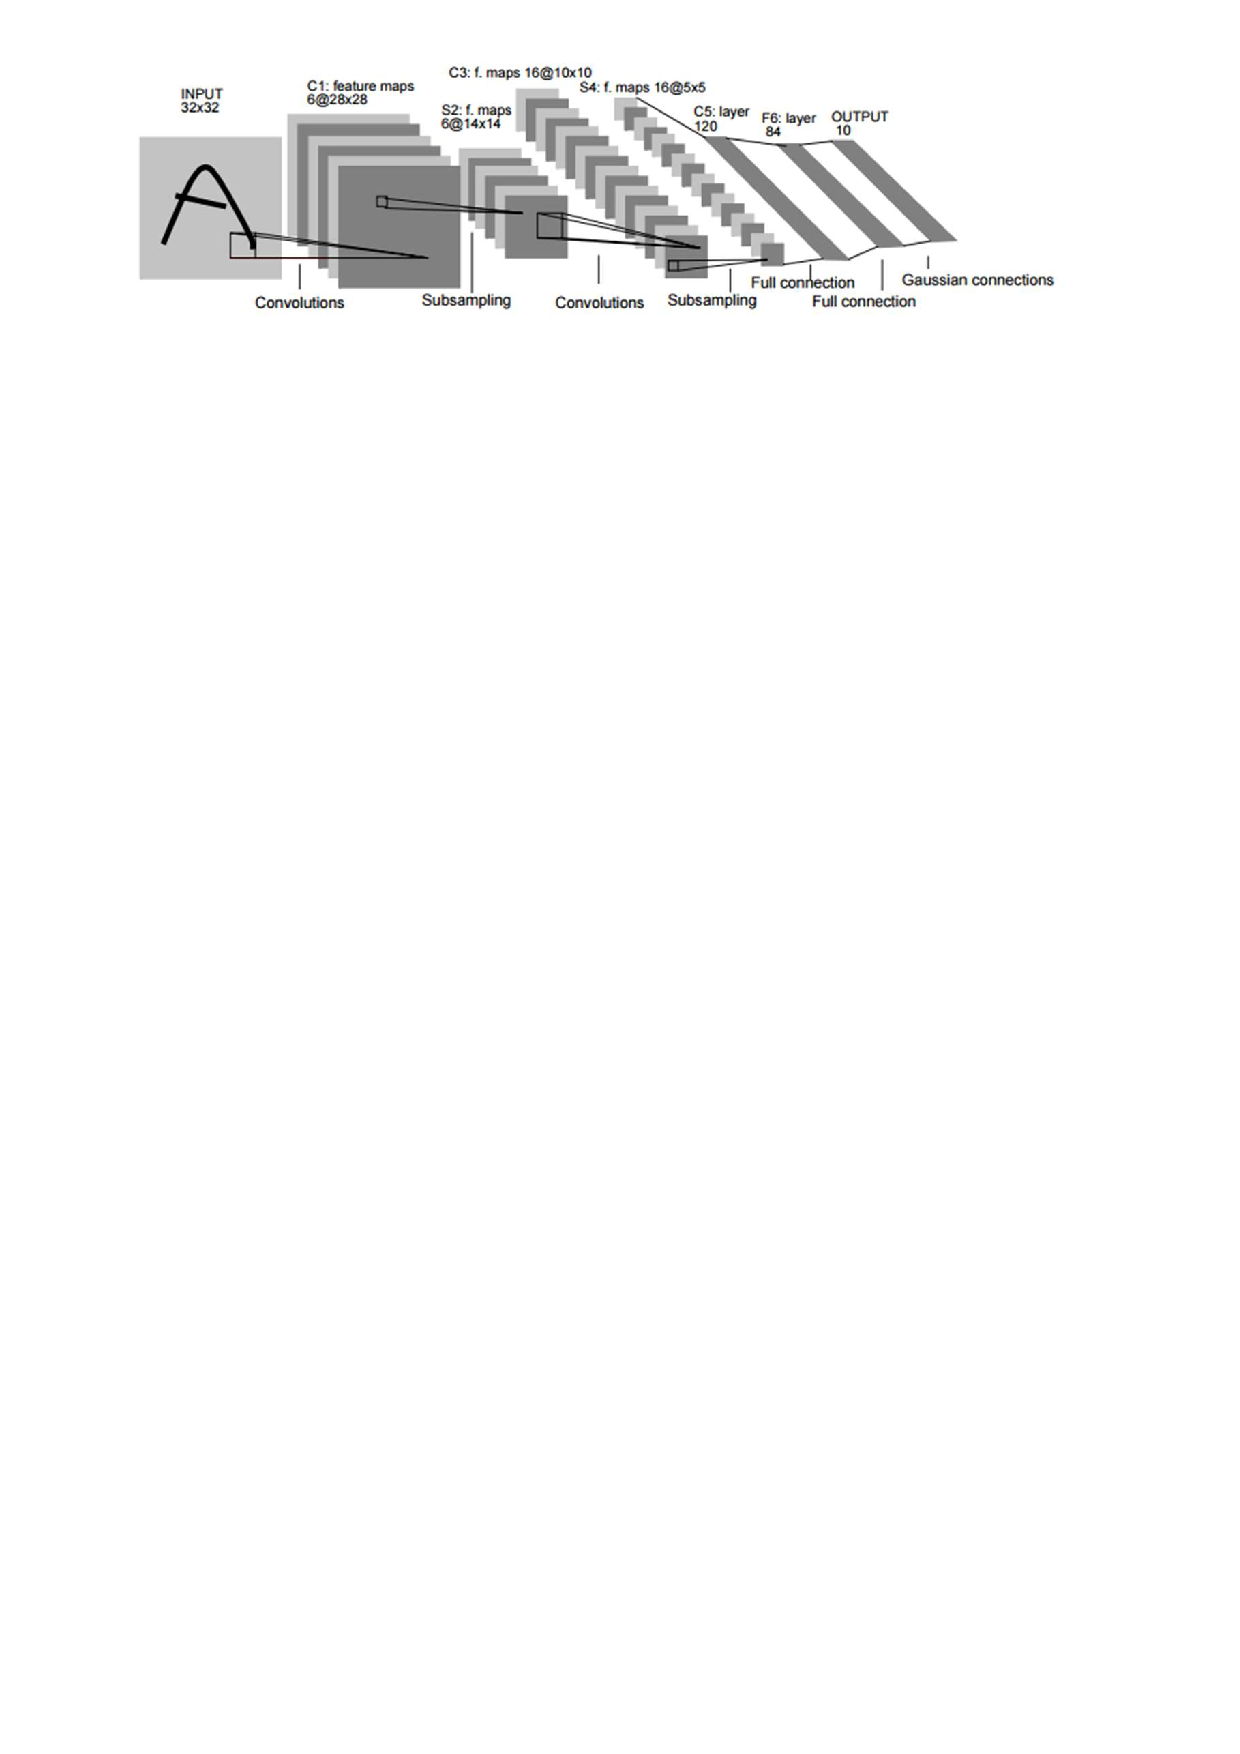
\includegraphics[trim=2cm 23cm 0cm 1cm]{figs/cnn.pdf}
	\caption{The architecture of a CNN example: LeNet5. Reprinted from \cite{cnn}.}
	\label{fig:cnn}
\end{figure}

\begin{figure}
	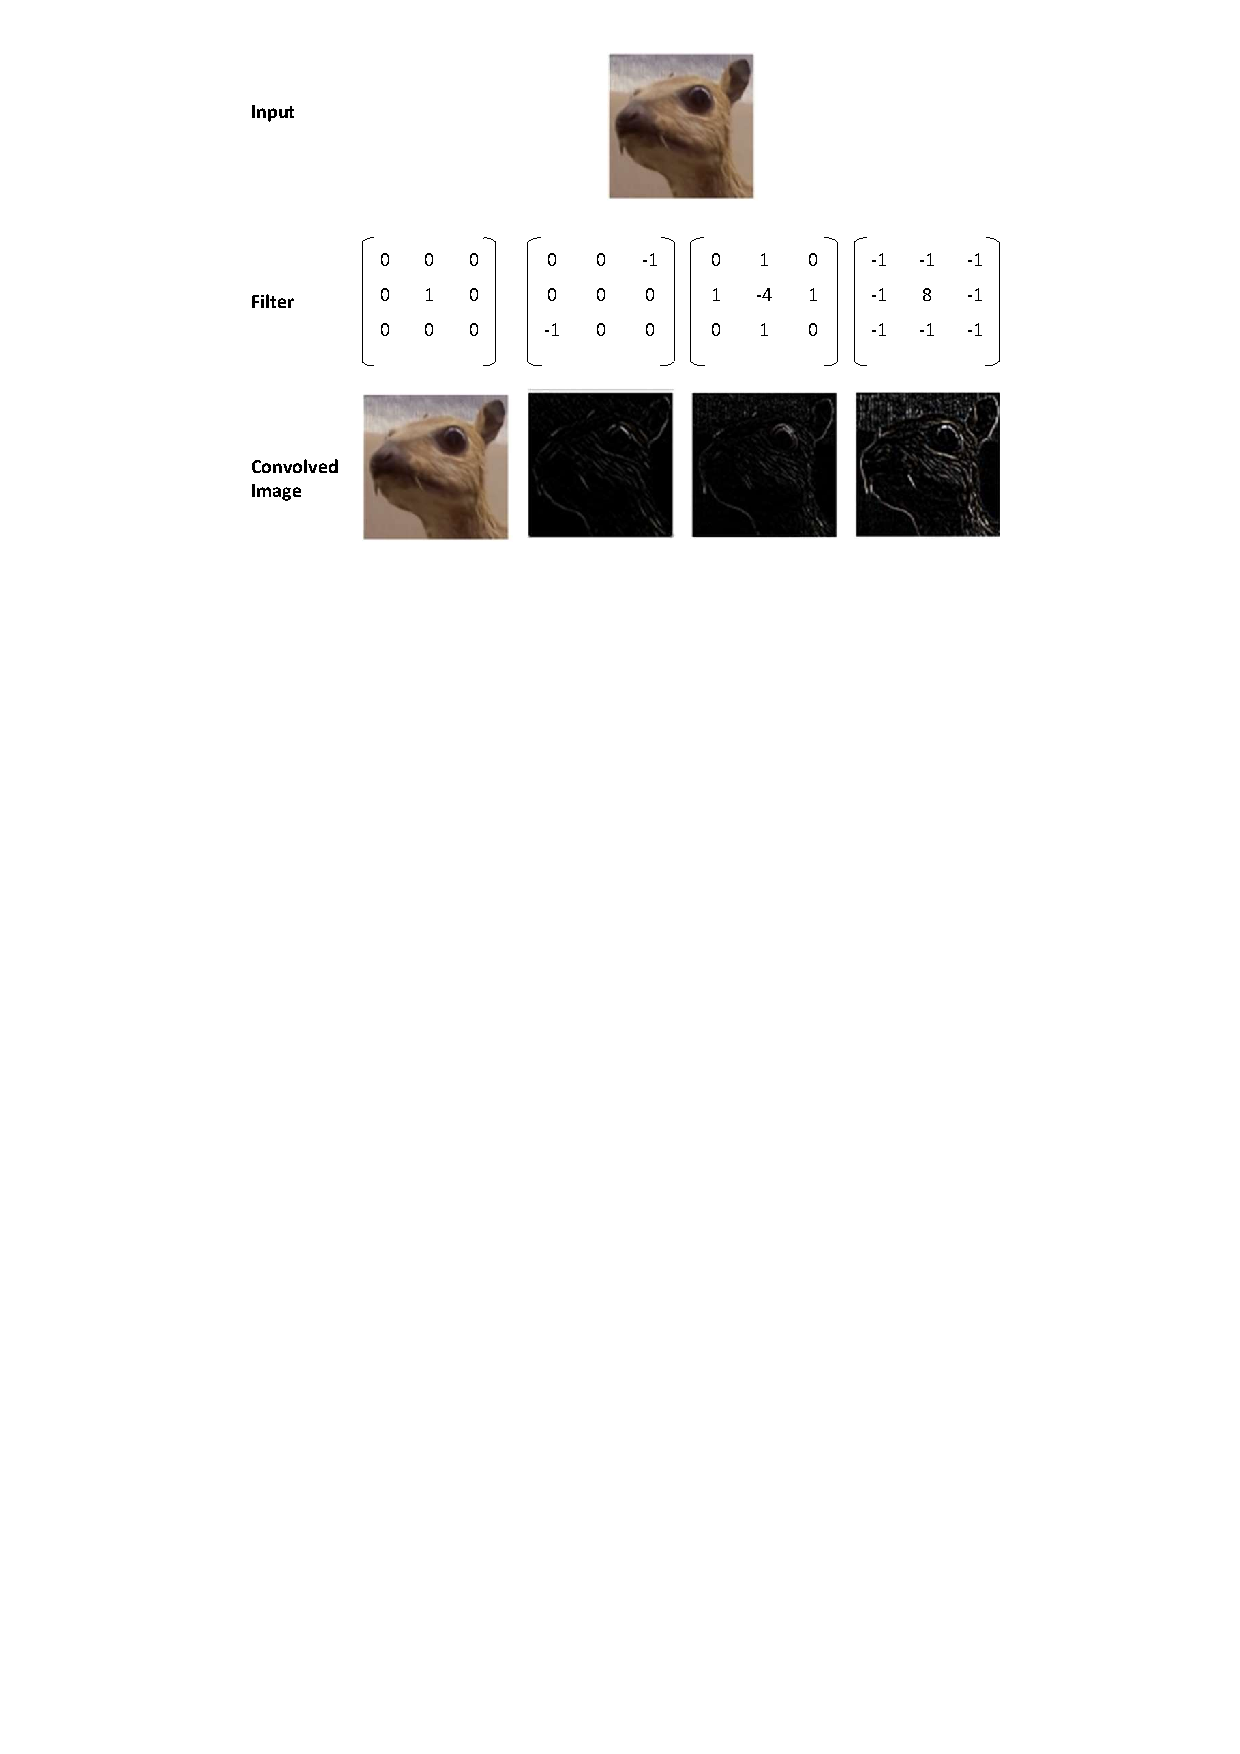
\includegraphics[trim=2cm 20cm 0cm 1cm]{figs/conv.pdf}
	\caption{The intuitive illustration of convolution over image.}
	\label{fig:conv}
\end{figure}
 
\par
There is related work \cite{ning2005} in the earlier stage which just simply applies CNN and treats videos as set of single frames and averages the results over all frames as the overall result. The performance of such method is not very satisfying since it doesn't take the important temporal information into consideration and there may be many irrelevant frames in the video will confuse the result. In recent years, many new related works are proposed to solve these problems, like Spatial-Temporal CNN\cite{karpathy2014}, Two-Stream ConvNet\cite{simonyan2014}, and 3D Convolutional Networks(3D-ConvNet) \cite{3dcnn_1} \cite{Ji2013} \cite{Tran2015}.  

\subsection{Spatial-Temporal CNNs feature descriptor}
\label{2_3_1}

Since spatial information represents the appearance and temporal information represents motion, they are both essential for video analysis. Karpathy et al. suggested a spatial-temporal CNN in their work\cite{karpathy2014}. They studied several approaches to extend the connectivity of CNNs to time domain to make use of spatial-temporal information of videos, including late fusion, early fusion and slow fusion. The architectures of fusion CNNs are illustrated in Figure \ref{fig:STCNNs}. 
\par 
Single frame architecture is used as a base-line in the work \cite{karpathy2014}. It is a standard CNNs framework and similar to the ImageNet challenge winning model \cite{kriz2012} just with the different input image resolution. The architecture of the single frame network is illustrated in Figure \ref{fig:STCNNs} (a).
\par 
Late fusion model, illustrated in Figure \ref{fig:STCNNs} (b), places two separate single frame networks which share network parameters. The inputs of two networks are two streams which have distance of 15 frames. The two networks are merged in the first fully connected layer. Neither single network alone can detect any motion, but the first full connected layer can compute global motion characteristics by comparing outputs of the two networks. 
\par 
Early fusion model, illustrated in Figure \ref{fig:STCNNs} (c), is similar to single frame model but the input is consecutive \(T\) frames instead of one single frame. \(T\) was set to \(10\) in the work \cite{karpathy2014}. The early and directly connectivity to pixel data allows the network to precisely detect local motion direction and speed.
\par 
The slow fusion model, illustrated in Figure \ref{fig:STCNNs} (d),  combines the early and late fusion model. This model slowly fuses temporal information throughout the network such that higher layers get access to progressively more global information in both spatial and temporal dimensions. 

\begin{figure}
	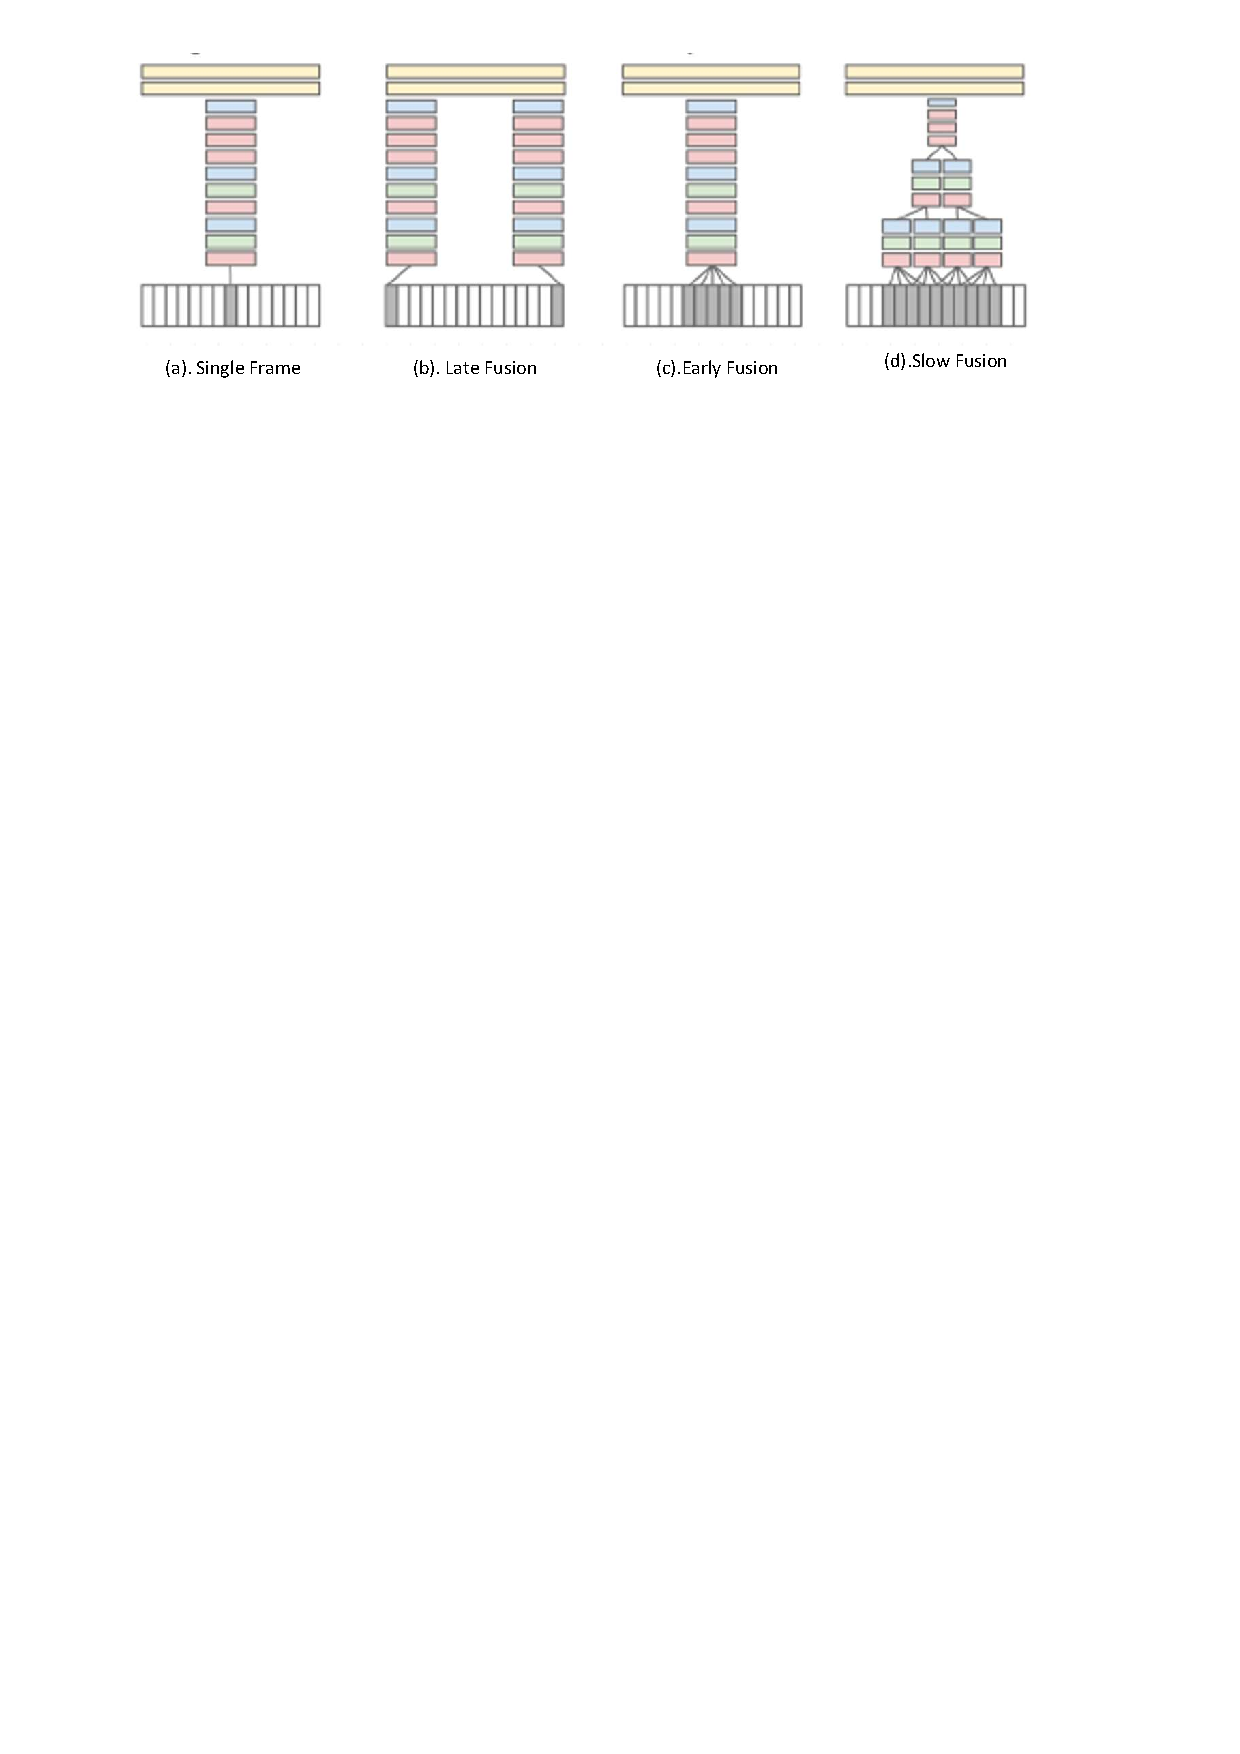
\includegraphics[trim=2cm 23cm 0cm 1cm]{figs/STCNNs.pdf}
	\caption{Explored approaches for fusing information over
		temporal dimension through the network. Red, green and
		blue boxes indicate convolutional, normalization and pooling
		layers respectively. In the Slow Fusion model, the depicted
		columns share parameters. Reprinted from \cite{karpathy2014}.}
	\label{fig:STCNNs}
\end{figure}

\subsection{Two-Stream ConvNet feature descriptor}
\label{2_3_2}
Two-Stream ConvNet proposed by Simonyan et al. \cite{simonyan2014} is another extension of ConvNet to action recognition in video data. The Two-Stream ConvNet introduces a different architecture with Spatial-Temporal CNNs \cite{karpathy2014} based on two separate recognition streams (spatial and temporal), which are combined by late fusion. The spatial stream learns appearance features from still video frames while the temporal stream learns motion features in the form of dense optical flow of input videos. So, the combination of spatial and temporal streams can represent both appearance/shape and motion for the input videos. The architecture of Two Stream ConvNet is illustrated in Figure \ref{fig:tsconvnet_1}.

\begin{figure}
	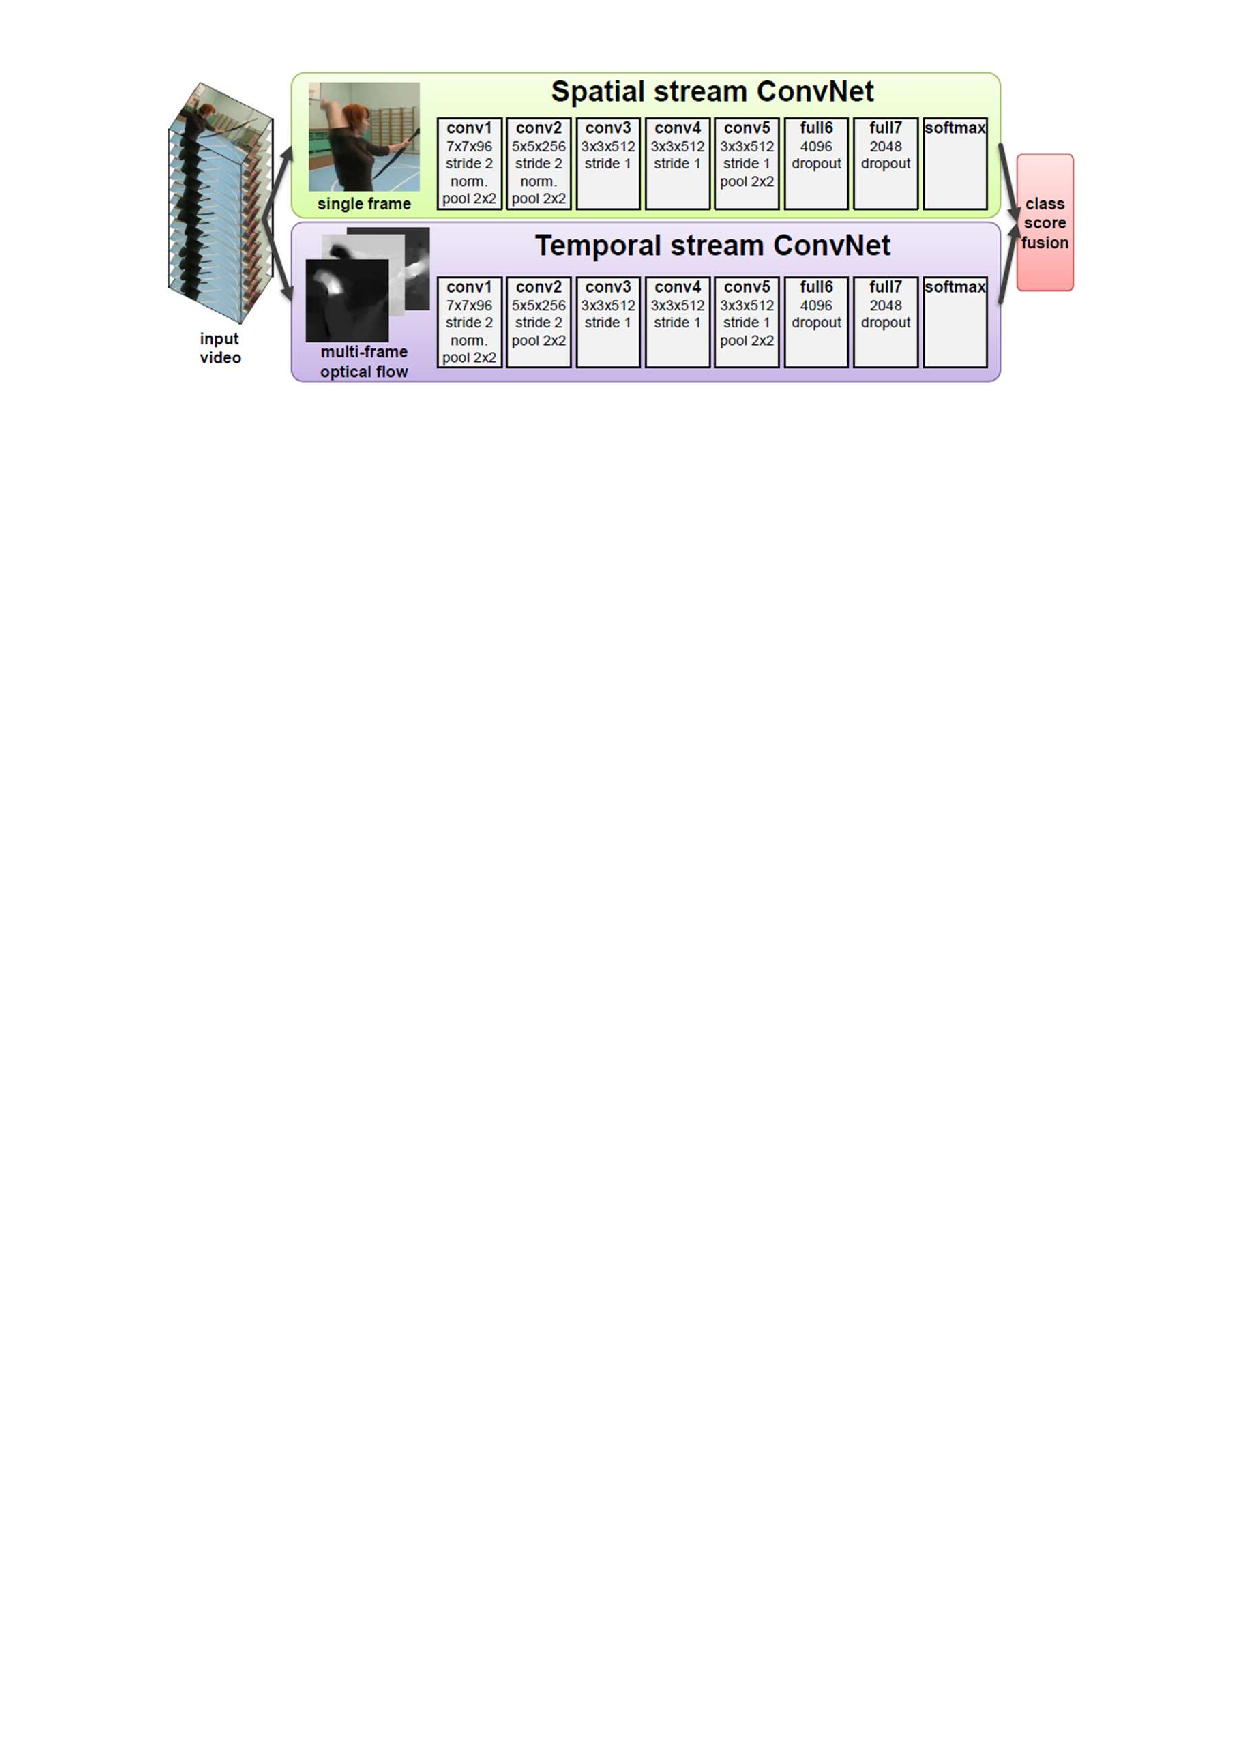
\includegraphics[trim=2cm 23cm 0cm 1cm]{figs/tsconvnet.pdf}
	\caption{The architecture of Two Stream ConvNet. Reprinted from \cite{simonyan2014}.}
	\label{fig:tsconvnet_1}
\end{figure}
   

\subsection{3D ConvNet feature descriptor}
\label{2_3_3}
3D ConvNet is first proposed by Ji et al. \cite{Ji2013} with human body segmented video volumes as input and Tran et al. \cite{Tran2015} improved it to accept full raw video volumes as input without any pre-processing. The main difference between 2D ConvNets and 3D ConvNets is the convolution and pooling are applied in three dimensions(x,y,time) instead of two(x,y). As illustrated in Figure \ref{fig:3DConv}, 2D convolution applied on a single image or a video volume (multiple frames as multiple channels) all result in an image. While 3D Convolution on a video volume results in another video volume. So, the video temporal information is lost after applying 2D convolution, while 3D convolution preserves both spatial and temporal information. 
\par 
The network architecture used in \cite{Tran2015} annotated as C3D is illustrated in Figure \ref{fig:3DConvNet}. The input of the network is a 16 frames video volume. Videos with frame number larger than 16 will be split into several 16 frames video clips with an overlap of 8 frames for each clip. All video clips for a video will calculate features separately and simply average them to get a 4096 dimensions features as the whole video's features. 
\par
The Figure \ref{fig:3DConvNetV} illustrates what the 3D ConvNet learns by using the deconvolution method explained in \cite{zeiler2014}. In the two examples, the features first focus on appearance and gradually track the motion over the rest of frames. 

\begin{figure}
	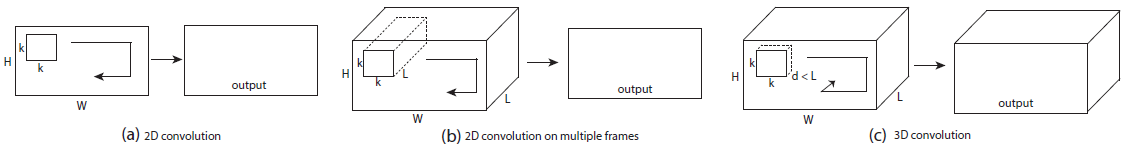
\includegraphics[width=\linewidth]{figs/3DConv.png}
	\caption{2D and 3D convolution operations. a) Applying 2D convolution on an image results in an image. b) Applying 2D convolution
		on a video volume (multiple frames as multiple channels) also results in an image. c) Applying 3D convolution on a video volume results
		in another volume, preserving temporal information of the input signal. Reprinted from \cite{Tran2015}.}
	\label{fig:3DConv}
\end{figure}

\begin{figure}
	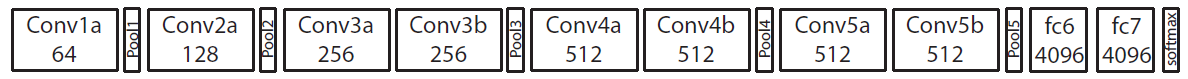
\includegraphics[width=\linewidth]{figs/3DConvNet.png}
	\caption{The architecture of C3D. C3D has 8 convolution, 5 max-pooling, and 2 full connected layers, followed by a softmax output layer. All 3D convolution kernels are \(3 \times 3 \times 3\) with stride 1 in both spatial and temporal dimensions. Number of filters are denoted in each box. The 3D pooling layers are denoted from pool1 to pool5. All pooling kernels are \(2 \times 2 \times 2\) except for pool1 is \(1 \times 2 \times 2\). Each fully connected layer has 4096 output units. Reprinted from \cite{Tran2015}.}
	\label{fig:3DConvNet}
\end{figure}

\begin{figure}
	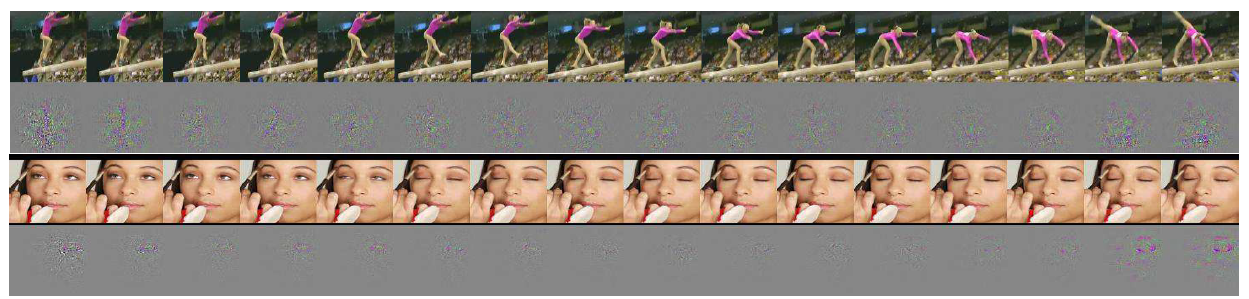
\includegraphics[width=\linewidth]{figs/3DConvNetV.png}
	\caption{Visualization of C3D model. Interestingly, C3D captures appearance for the first few frames but thereafter only attends to salient motion. Reprinted from \cite{Tran2015}.}
	\label{fig:3DConvNetV}
\end{figure}

\section{Datasets}
\label{2_4}

Training dataset is one of the key factors to train a high performance feature descriptor. At the same time, published and widely used datasets can be helpful to compare between different approaches. After the publication of the KTH \cite{kth} dataset which contains 6 action classes and 600 videos (2391 sequences) in 2004, more and more human activity datasets were published. In recent years, the development of dataset has the following characteristics:
\begin{enumerate}
	\item More action classes, the KTH has 6 classes, UCF101 \cite{ucf101} has 101 action classes and ASLAN \cite{aslan} has 432 classes.
	\item More training and testing samples, KTH has 192 videos for training and 216 videos for testing while ActivityNet \cite{activitynet200} 200 has 10024 videos for training and 5044 videos for testing.
	\item The video scene becomes more and more complex, KTH is acted by limited number of actors, while recent datasets are cut from realistic scenes, like youtube, cctv, BBC etc.
	\item More challenges in video content, from fixed backgrounded without camera motion to  non-static camera, multi-viewpoints, more complex background; from single person action to  human-human interaction, human-object interaction, etc.    
\end{enumerate}  

\subsection{List of human activity video datasets}
Part of widely used action and interaction video datasets are illustrated in Table \ref{table:action_datasets} and Table \ref{table:interaction_datasets} respectively.
\begin{table}
	\caption{List of human action video datasets}
	\begin{center}
		\begin{tabular}{| p{2.5cm} | p{1.5cm} | p{4cm} | p{3cm} | p{4cm} |}
			\hline
			Dataset & Classes & Videos & Annotations & Properties \\ \hline \hline
			% *********************************************************************
			% KTH 
			% *********************************************************************
			KTH\cite{kth} 
			& % classes
			6 action classes 
			& % videos 
			\vspace{-5mm}
			\begin{myitemize}
				\item Training : 192
				\item Validation: 192
				\item Testing: 216
				\item Resolution: \(160 \times 120\) @ 25fps
			\end{myitemize}
            & % anotations
			\vspace{-5mm}
			\begin{myitemize}
				\item Action labels
				\item Temporal segments
			\end{myitemize}
	    	& %properties
	    	\vspace{-5mm}
	    	\begin{myitemize}
	    		\item Static camera
	    		\item Simple background
	    		\item Acted by 25 subjects, 6 actions and 4 scenarios
	    	\end{myitemize}
    		\\ \hline 
	    	
	    	% **********************************************************************
	    	% Hollywood2
	    	% **********************************************************************
	    	Hollywood2\cite{marszalek09}
	    	& % classes
	    	12 action classes and 10 scene classes
	    	& % videos 
	    	For actions:
	    	\vspace{-3mm}
	    	\begin{myitemize}
	    		\item Training : 823
	    		\item Testing: 884	
	    	\end{myitemize}
    		For scenarios:
    		\vspace{-3mm}
    		\begin{myitemize}
    			\item Training : 570
    			\item Testing: 582	
    		\end{myitemize}
    		Resolution: \(400-300 \times 300-200\)
	    	& % anotations
	    	\vspace{-5mm}
	    	\begin{myitemize}
	    		\item Action labels
	    		\item Scene labels
	    	\end{myitemize}
	    	& %properties
	    	\vspace{-5mm}
	    	\begin{myitemize}
	    		\item Non-static camera
	    		\item Realistic scenarios from movies
	      	\end{myitemize}
	    	\\ \hline 


	    	% **********************************************************************
	    	% UCF101
	    	% **********************************************************************
	    	UCF101\cite{ucf101}
	    	& % classes
	    	5 types, 101 action classes
	    	& % videos 
	    	\vspace{-5mm}
	    	\begin{myitemize}
	    		\item Training : 9537
	    		\item Testing: 3783
	    		\item Resolution: \(400-300 \times 300-200\)	
	    	\end{myitemize}
	    	
	    	& % anotations
	    	\vspace{-5mm}
	    	\begin{myitemize}
	    		\item Action labels
	    	\end{myitemize}
	    	& %properties
	    	\vspace{-5mm}
	    	\begin{myitemize}
	    		\item Realistic scenarios from YouTube
	    		\item Large variations in camera motion, object appearance and pose, object scale, viewpoints, cluttered background, illumination conditions, etc.
	    	\end{myitemize}
	    	\\ \hline
	    	
	    	
	    	% **********************************************************************
	    	% ActivityNet
	    	% **********************************************************************
	    	ActivityNet 200\cite{activitynet200}
	    	& % classes
	    	200 action classes
	    	& % videos 
	    	\vspace{-5mm}
	    	\begin{myitemize}
	    		\item Training : 10024
	    		\item Validation: 4926
	    		\item Testing: 5044
	    	\end{myitemize}
	    	
	    	& % anotations
	    	\vspace{-5mm}
	    	\begin{myitemize}
	    		\item Action labels
	    		\item Temporal segments
	    		\item Hierarchy activities relationship
	    	\end{myitemize}
	    	& %properties
	    	\vspace{-5mm}
	    	\begin{myitemize}
	    		\item Realistic scenarios
	    		\item Large variations in camera motion, object appearance and pose, object scale, viewpoints, cluttered background, illumination conditions, etc.
	    	\end{myitemize}
	    	\\ \hline
   	
		\end{tabular}
		\label{table:action_datasets}
	\end{center}
\end{table}

\begin{table}
	\caption{List of human interaction video datasets}
	\begin{center}
		\begin{tabular}{| p{2.5cm} | p{1.5cm} | p{4cm} | p{3cm} | p{3cm} |}
			\hline
			Dataset & Classes & Videos & Annotations & Properties \\ \hline \hline
			
			% **********************************************************************
			% UT-Interaction
			% **********************************************************************
			UT-Interaction\cite{ut2010}
			& % classes
			6 interaction classes
			& % videos 
			\vspace{-5mm}
			\begin{myitemize}
				\item 20 videos
				\item 2 sets, 10 for each set. Evaluated by leave one out cross validation.
				\item Resolution = \(720 \times 480\)
			\end{myitemize}
			
			& % anotations
			\vspace{-5mm}
			\begin{myitemize}
				\item Interaction labels
				\item Temporal segments
				\item Spatial segments
			\end{myitemize}
			& %properties
			\vspace{-5mm}
			\begin{myitemize}
				\item Two-person interaction
				\item Static camera
				\item Acted in different background
			\end{myitemize}
			\\ \hline
			
			% **********************************************************************
			% ShakeFive2
			% **********************************************************************
			ShakeFive2\cite{shakefive2}
			& % classes
			8 interaction classes
			& % videos 
			\vspace{-5mm}
			\begin{myitemize}
				\item 153 videos
				\item Resolution = \(1280 \times 720\)
			\end{myitemize}
			
			& % anotations
			\vspace{-5mm}
			\begin{myitemize}
				\item Interaction labels
				\item Joint position
				\item Temporal segments
			\end{myitemize}
			& %properties
			\vspace{-5mm}
			\begin{myitemize}
				\item Homogeneous background 
				\item Static camera
			\end{myitemize}
			\\ \hline
			
			% **********************************************************************
			% MMI
			% **********************************************************************
			Multi-modal \& Multi-view \& Interactive \cite{m2i_tju}
			& % classes
			9 interaction classes and 13 person-object interaction classes
			& % videos 
			\vspace{-5mm}
			\begin{myitemize}
				\item 1760 RGB videos
				\item 1760 depth videos
				\item Resolution = \(320 \times 240\)
			\end{myitemize}
			
			& % anotations
			\vspace{-5mm}
			\begin{myitemize}
				\item Interaction labels
				\item Joint position
				\item Foreground mask
			\end{myitemize}
			& %properties
			\vspace{-5mm}
			\begin{myitemize}
				\item Homogeneous background 
				\item Static camera
			\end{myitemize}
			\\ \hline
			
			
		\end{tabular}
		\label{table:interaction_datasets}
	\end{center}
\end{table}

%=========================================================